\iffalse

References draft:

Jaeyoung Choi, Jack J. Dongarra, David W. Walker.  Parallel Matrix Transpose Algorithms on Distributed Memory Concurrent Computers.  Mathematical Sciences Section Oak Ridge National Laboratory P.O. Box 2008, Bldg. 6012 Oak Ridge, TN 37831-6367
- Notes: The communication is based of the greatest commond divisor (GCD) of the number of rows and columns (P and Q). If P and Q are relatively prima, the matrix transpose algorithm involves complete exchange communication. A block is LCM/P x LCM/Q if not relativaly prime and only LCM/GCD communications are required.
- The algorithms make use of non-blocking, point-to-point communication between proces-
sors. The use of nonblocking communication allows a processor to overlap the messages that it sends to different processors, thereby avoiding unnecessary synchronization.

Jonathan Eckstein, Gyorgy Matyasfalvi. Efficient Distributed-Memory Parallel Matrix-Vector Multiplication with Wide or Tall Unstructured Sparse Matrices.
- on sparse matrixes, but Its about vector multiplications

John C. Bowman, Malcolm Roberts. Adaptive Matrix Transpose Algorithms for Distributed Multicore Processors.
- really nice for my problem
- hybrid approach with both shared and distributed
- Notes: "The most popular algorithms for transposing an NxN matrix distributed over P processes are the direct communicatoin (all-to-all, simpler implementation) and recursive binary exchange (butterfly) algorithms."

Jaeyoung Choi, Jack Dongarra, David W. Walker. The design of scalable software libraries for distributed memory concurrent computers. Oak Ridge National Laboartory Mathematical Sciences Section. Oak RIdge, TN 37831-6367.
- they explained (apparently) block cyclic data distribution. Actually no


So we learned that block cyclic data distribution (round robin) is efficient for data access. You can mix blocks with cycles to get a few combinations to try out.

Sheng Ma, Libo Huang, Mingche Lai, Wei Shi. Network-on-chip customizations for message passing interface primitives: From Implementations to Programming Paradigms, 2015
- In conventional MPI implementations, MPI_Bcast is typically implemented using software with a tree-based algorithm. Such implementations exploit point-to-point communication operations. Thus, the number of hops to reach leaf nodes increases with the total number of nodes (typically in a logarithmic manner); the latency of MPI_Bcast also increases.
- this is useful in the findings because we find the same outcome
- but I use scatter and gather... i should look at the implementation

From the source code: coll/coll_base_scatter:
- There are 3 implementations of scatter:
  - binomial tree algorithm, as discussed above uses point-to-point communications
  - linear functions which work the same for small values
  - linear non blocking
- The decision is taken in coll/tuned/coll_tuned_scatter_decision.c

GPU:
J. Gómez-Luna, I. -J. Sung, L. -W. Chang, J. M. González-Linares, N. Guil and W. -M. W. Hwu, "In-Place Matrix Transposition on GPUs," in IEEE Transactions on Parallel and Distributed Systems, vol. 27, no. 3, pp. 776-788, 1 March 2016, doi: 10.1109/TPDS.2015.2412549. 

Wonderful paper about cache:
S. Chatterjee and S. Sen, "Cache-efficient matrix transposition," Proceedings Sixth International Symposium on High-Performance Computer Architecture. HPCA-6 (Cat. No.PR00550), Touluse, France, 2000, pp. 195-205, doi: 10.1109/HPCA.2000.824350.

\fi


\documentclass[conference]{IEEEtran}
\IEEEoverridecommandlockouts
% The preceding line is only needed to identify funding in the first footnote. If that is unneeded, please comment it out.
\usepackage{cite}
\usepackage{blindtext}  % generate random text
\usepackage{amsmath,amssymb,amsfonts}
\usepackage{algorithm}
% \usepackage{algorithmic}
\usepackage{graphicx}
\usepackage{textcomp}
\usepackage{xcolor}
\usepackage{algpseudocode}
\usepackage{graphicx}
\usepackage{hyperref}
\usepackage{booktabs} % table

\def\BibTeX{{\rm B\kern-.05em{\sc i\kern-.025em b}\kern-.08em
    T\kern-.1667em\lower.7ex\hbox{E}\kern-.125emX}}
\begin{document}

\title{Comparing shared and distributed memory algorithms: A case study on Matrix Transposition and Symmetry Check\\
%{\footnotesize \textsuperscript{*}Note: Sub-titles are not captured in Xplore and
%should not be used}
%\thanks{Identify applicable funding agency here. If none, delete this.}
}

\author{\IEEEauthorblockN{Giovanni Santini}
\IEEEauthorblockA{\textit{University of Trento}\\
Trento, Italy \\
giovanni.santini@studenti.unitn.it \\
MAT. 235441 \\
\href{https://github.com/San7o/parallel-computing-cpp}{github.com/San7o/parallel-computing-cpp}}
}

\maketitle

\begin{abstract}
This study evaluates matrix transposition on shared- and distributed-memory
architectures, focusing on scalability. The shared-memory implementation
achieves optimal linear strong scaling for matrixes of size $N<2^{10}$,
while distributed-memory implementations are hindered by communication overhead, with
\textit{matTransposeMPIBlock} performing better then the seqencial
implementation only on big matrixes, but scaling well on big matrices.
Weak scaling is poor for all implementations, though the shared-memory
approach is slightly more efficient. Shared-memory systems are ideal
for moderate problem sizes, while distributed-memory systems trade
efficiency for scalability with larger matrices.
\end{abstract}

\begin{IEEEkeywords}
parallel computing, matrix transpose, symmetric matrix, benchmark
\end{IEEEkeywords}

\section{Introduction}

Shared-memory systems are widely used in performance-critial applications
to leverage multiple CPU cores on the same machine.
There are, however, limitations to this approach due to all CPU cores
competing for access to memory over a shared bus, which creates contention
and reduces performance. Additionally, scaling the number of cores in
shared-memory systems is challenging. Consequently, distributed-memory
models are widely used, as they allow memory operations to be
distributed across multiple computing nodes, and the system can
be scaled by adding new nodes to the cluster. While distributed-memory
systems offer significant advantages, they
depend on the network layer to exchange information, which can
introduce network latency and bandwidth saturation as potential
bottlenecks. To mitigate these challenges, technologies such as
InfiniBand \cite{b0}, RDMA \cite{b-1} and local caching \cite{b-2}
aim to minimize communication overhead and
enhance data transfer efficiency. Modern MPI implementations,
including OpenMPI and MPICH2, are optimized to utilize these
technologies \cite{b1} \cite{b2}, enabling improved performance in
distributed-memory environments. The two memory models each
have distinct strengths and limitations,
making a comparison between the two essential for evaluating optimal
system performance. In this report, an implementation of \textit{matTranspose}
and \textit{checkSymm} is presented on distributed-memory systems using MPI.
This implementation is then compared with a shared-memory counterpart
developed using OpenMP. Additionally, various compiler
optimization strategies are discussed.

The rest of the report is organized as follows.
In section 2, we discuss the state of the art of the two algorithms.
In section 3, we elaborate on the algorithms analyzed.
In section 4, we explain the benchmarking procedures and system
information. In section 5, we present the results. The conclusion
is in section 6. Section 7 contains the project's github link

\section{State of the Art}

\iffalse
- Parallel Matrix Transpose Algorithms on Distributed Memory Concurrent
  Computers
- Adaptive Matrix Transpose Algorithms for Distributed Multicore Processors
- Efficient Distributed-Memory Parallel Matrix-Vector Multiplication with
  Wide or Tall Unstructured Sparse Matrices.
- In-Place Matrix Transposition on GPUs

\fi

Distributed-memory matrix transposition is a well discussed problem.
Choi, Dongarra and Walker \cite{b3} presented an implementation
based on the block cyclic data distribution. In their approach, the
matrix is divided into blocks of arbitrary size. If the numbers of rows and
columns are relatively prime, then the algorithm consists of a two-dimension
complete exchange of information where each processor sends a sub block
to every other processor. Binary exchange was shown to be the faster communication
scheme \cite{b4} which completes the exchange in $log_2 P$ steps where
$P$ is the number of processors. If the number of rows and columns
are not relatively prime, processors are grouped into a number of groups
equal to the greatest common divisor of the number of rows and columns, and
communication is overlapped between groups using
non-blocking point-to-point communication. Bowman and Roberts \cite{b5} later
presented an hybrid approach leveraging both shared and distributed memory.
Eckstein and Matyasfalvi
\cite{b6} studied the distributed problem on wide or tall unstructured sparce matrices.
Their implementation assignes nonzero elements of the matrix evenly
between processes by partitioning the matrix by sections of non zero
elements of the same length. Juan Gómez-Luna et. al. \cite{b7} presented
several GPU applications and an heuristic to detect the optimal approach.

\section{Contribution and Methodology}

Since both \textit{matTranspose} and \textit{checkSymm} are memory bounded
\cite{b10}, most of the time is expected to be spent on memory movement rather then
math operation. Implementations with MPI distribute the matrix over the network,
potentially creating a bottleneck by adding additional latency due to
synchronyzation, the overhead of the operative system's network stack and
network congestion. Practically the number of computing nodes
in a cluster could greately surpass the number of CPU cores of a
shared-memory computer therefore overcoming the disadvantages and
possibly increasing the performance by dividing the work in a greater
number of workers, however the advantages could be shadowed by the
memory movement memory bounded algorithms. On the other hand, shared-memory
algorithms do not need to send memory since they share the same address
space and are limited by the bus bandwidth and scheduling policies.
In this section, implementations of both \textit{matTranspose}
and \textit{checkSymm} using MPI are presented, starting with
\textit{matTranspose}. We benchmark the bandwidth and speedup
of different MPI implementations compared to a serial and to a OpenMPI one,
discussing weak and strong scaling. Different compiler optimizations
will also be compared. All benchmarks will be tested against every
matrix size from $2^2$ to $2^{12}$, we will assume the number of processes
is divisible by the matrix size and the square root is an integer
number for ease of implementation, however the algorithms can be
generalised with few modifications. The algorithms for \textit{matTranspose}
will now be explained.

\textit{matTranspose} takes a $N \times N$ input square matrix
\textit{input}, a matrix of the same shape \textit{ouput}, and the
size of the two matrices \textit{size}. The analyzed algorithms are the following:
\begin{itemize}
\item \textit{matTranspose}: naive implementation of matTranspose,
iterating over values of the input matrix and storing them in the
output matrix with indexes of rows and columns swapped.
\item \textit{matTransposeMPI}: this implementation takes full advantage
  of MPI datatypes to test bandwidth. Leveraging 
  custom datatypes in MPI, \textit{MPI\_Type\_contiguous} was used
  to define a row type and \textit{MPI\_Type\_vector} + \textit{MPI\_Type\_create\_resized}
  for a column type. The root process scatters rows with \textit{MPI\_Scatter} and
  retrieves columns with \textit{MPI\_Gather}, therefore
  transposing the matrix. Each process receives a block of rows and
  sends back the same block to the root but as column type. The algorithm
  automatically assign the correct number of rows/column to each process based on the
  number of processes so that the entire matrix is transposed.
  For example, in a $16x16$ matrix with $4$ processes, each processes
  receives $\frac{16}{4}=4$ rows and sends the same number back as
  columns.
  This implementation fully tests the communication
  bandwidth and latency by relying only on communication and MPI
  functionalities.
\item \textit{matTransposeMPIBlock}: this implementation divides the
  original matrix into a mesh of square sub-matrixes with side length equal to
  $\frac{N}{\sqrt{\#processes}}$ using MPI datatypes. Each sub-matrix is assigned
  to a different processes. The root process sends the sub-matrix to the
  other processes with \textit{MPI\_Scatterv} and receives the same
  number of sub-matrices but in transposed order with \textit{MPI\_Gatherv},
  for example process[0][1] will sand to root[1][0].
  Each process tranposes its sub-matrix and sends It back to the root.
  This approach tests a different communication method.
\item \textit{matTransposeOMPX}: this set of algorithms are all derived
  from \textit{matTranspose} with the outer for loops parallelized using
  omp with the number of threads \textit{X} being a power of 2 from $2^1$ to $2^6$.
\end{itemize}
The algorithm for \textit{checkSymm} will now be explained. The algorithm
takes an $N \times N$ square matrix \textit{input}, a size \textit{size}
and returns true if the matrix is symmetrix, false otherwise.
The algorithm the following:
\begin{itemize}
\item \textit{checkSymm}: naive implementation of checkSymm. It
Iterates over the upper half of the matrix and testing if every value
is equal to the symmetric value.
\item \textit{checkSymmMPI}: similar to \textit{matTransposeMPIBlock},
but each process receives both a sub-matrix and the transposed sub-matrix,
that is, if we treated each sub-matrix as a single element of a matrix,
the element in the tranposed position will be received. Each process
compares the two sub-matrices to check if they are symmetric. The
result is computed
via \textit{MPI\_Reduce}.
\item \textit{checkSymOMPX}: similar to \textit{matTransposeOMPX} but
based on \textit{checkSymm}. After each parallel section, a barrier
is needed to synchronize the shared boolean output variable.
\end{itemize}

\textit{Strong Scaling} or \textit{Speedup} is defined as the reatio
between the time for running the algorithm using one processor $t(1)$ over
the time for running the same algorithm on $N$ processors $t(N)$ \ref{eq:1}.
\begin{equation} \label{eq:1}
Speedup = \frac{t(1)}{t(N)}
\end{equation}
In an ideal scenario, software would achieve a linear increase in
speed proportional to the number of processors used (speedup = N),
signifying that each processor is fully utilizing its computational
capacity.
In case of \textit{Weak Scaling}, both the number of processors $p$
and the problem size $N$ are increased \ref{eq:2}. It evaluates wheter a program
can handle larger problems efficiently when more resources are available.
\begin{equation} \label{eq:2}
S_w = \frac{t(N)}{T_p(N*p)}
\end{equation}


\section{Experiments and System Description}

\iffalse
- Detailed description of the computing system and platform. \\
- Relevant specifications or configurations (e.g., libraries
and programming toolchains). \\
- Description of the experimental setup, procedures, and
methodologies used in the project. \\
- Discussion on how experiments are designed to test the hypotheses
or achieve the objectives \\
\fi

Experiments were conducted on a cluster with 96 Intel(R) Xeon(R) Gold
6252N CPUs (2.30GHz) featuring 32K L1d and L1i caches, 1022K L2 cache,
36608K L3 cache (64-bit cache lines), 1 thread per core, and 4GB RAM,
running Linux 3.10. The algorithms were benchmarked using \textit{valFuzz},
with benchmarks compiled using gcc-9.1.0. Four benchmark sets were
compiled with different optimization levels: none, -O1, -O2 and "-O3
-Ofast -march=native".
MPI algorithms were benchmarked with number of processes equal to 4, 16, 64.
MPI benchmarks are composed of a master (root) process and a fleet
of worker processes. Before each benchmark, the master sends
a synchronization message to the workers telling them which algorithm
to execute and how many times, It will then start executing the agreed
algorithm and partecipate in the work. Only the master process will be
timed, recording wall-clock execution time statistics: minimum, maximum,
median, mean, standard deviation, Q1, and Q3. To ensure statistical
significance, each benchmark was executed 10 times. Cache interference was
minimized by clearing it before each run by writing to an array twice
the L3 cache size. Input matrices, consistent across algorithms, were
initialized with uniformly random floats (-1 to 1) generated via a
Linear Congruential Generator (LCG) \cite{b8} with parameters a=1664525,
c=1013904223, m=232 \cite{b9}, and seed 1337.
To expedite random number generation, values were precomputed at
compile time using \textit{tenno-tl}. Additional \textit{tenno-tl}
features, such as ranges and arrays, were also employed.

\section{Results and Discussion}

\begin{figure}[htb]
	\centering
	\includegraphics[width=0.44\textwidth]{"../benchmarks/plotting/images/matTransposeMPI_base.pdf"}
	\caption{matTransposeMPI average time over matrix size of multiple number of processes}
	\label{fig:transpose_mpi_base}
\end{figure}

\begin{figure}[htb]
	\centering
	\includegraphics[width=0.44\textwidth]{"../benchmarks/plotting/images/matTransposeMPI_block_base.pdf"}
	\caption{matTransposeMPIBlock average time over matrix size of multiple number of processes}
	\label{fig:transpose_mpi_block}
\end{figure}

\begin{figure}[htb]
	\centering
	\includegraphics[width=0.44\textwidth]{"../benchmarks/plotting/images/matTransposeMPI_speedup.pdf"}
	\caption{matTransposeMPI speedup measurements of multiple number of processes}
	\label{fig:transpose_mpi_speedup}
\end{figure}

\begin{figure}[htb]
	\centering
	\includegraphics[width=0.44\textwidth]{"../benchmarks/plotting/images/matTransposeMPI_block_speedup.pdf"}
	\caption{matTransposeMPIBlock speedup measurements of multiple number of processes}
	\label{fig:transpose_mpi_block_speedup}
\end{figure}

\begin{figure}[htb]
	\centering
	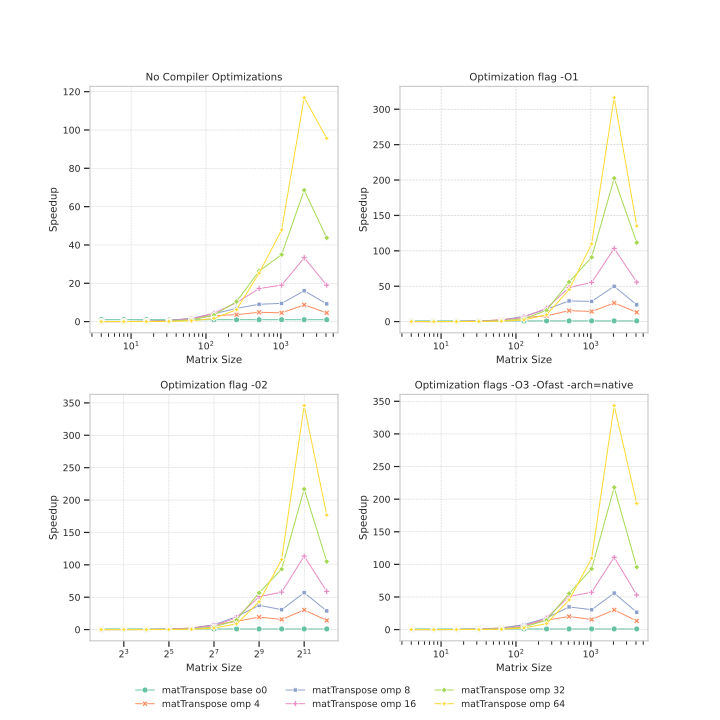
\includegraphics[width=0.44\textwidth]{"../benchmarks/plotting/images/transpose_explicit_speedup.pdf"}
	\caption{matTransposeOMP speedup}
	\label{fig:transpose_mp_speedup}
\end{figure}


\iffalse
\begin{figure}[htb]
	\centering
	\includegraphics[width=0.44\textwidth]{"../benchmarks/plotting/images/matTransposeMPI_weak_scaling.pdf"}
	\caption{matTransposeMPI weak scaling measurements of multiple number of processes}
	\label{fig:transpose_mpi_weak_scaling}
\end{figure}
\fi

\iffalse
\begin{figure}[htb]
	\centering
	\includegraphics[width=0.44\textwidth]{"../benchmarks/plotting/images/matTransposeMPI_block_bandwidth.pdf"}
	\caption{matTransposeMPIBlock bandwidth measurements of multiple number of processes}
	\label{fig:transpose_mpi_block_bandwidth}
\end{figure}
\fi

\iffalse
\begin{figure}[htb]
	\centering
	\includegraphics[width=0.44\textwidth]{"../benchmarks/plotting/images/matTransposeMPI_block_weak_scaling.pdf"}
	\caption{matTransposeMPIBlock weak scaling measurements of multiple number of processes}
	\label{fig:transpose_mpi_block_weak_scaling}
\end{figure}
\fi

\begin{figure}[htb]
	\centering
	\includegraphics[width=0.44\textwidth]{"../benchmarks/plotting/images/matTransposeMPI_block_weak_scaling_final.pdf"}
	\caption{Comparison of weak scaling between all the matTranspose implementations, averaging all the compiler optimization flags}
	\label{fig:transpose_mpi_block_weak_scaling_final}
\end{figure}


\begin{table}[h!]
\centering
\caption{Average time \% spent on each part of \\
\textit{matTransposeMPIBlock}}
\label{tab:normalized_averages}
\begin{tabular}{lc}
\toprule
\textbf{Column} & \textbf{Average Time \%} \\
\midrule
Displacement    & 0.000088 \\
Setup           & 0.000246 \\
Scatter         & 0.372926 \\
Transpose       & 0.149277 \\
Gather          & 0.477462 \\
\midrule
\end{tabular}
\end{table}

The results of the study are presented here. Shared-memory performance
data referenced in this analysis are derived from previous work \cite{b10}.

As discussed earlier, the memory-bound nature of both \textit{matTranspose}
and \textit{checkSymm} inherently disadvantages the distributed-memory
implementation when compared to the shared-memory approach due to its
higher memory movement requirements. Experimental results confirm this
observation. In the case of \textit{matTransposeMPIBlock}, a significant
portion of the execution time is consumed by data transmission
(approximately 37\%) and data reception (approximately 47\%), as shown
in Table~\ref{tab:normalized_averages}. This behavior accounts for the
slightly slower performance of \textit{matTransposeMPI} relative to the
sequential implementation (Figure~\ref{fig:transpose_mpi_base}) and the
considerably slower performance compared to the shared-memory OpenMP
implementation for $N > 2^7$. However, as the matrix size increases,
the performance of \textit{matTransposeMPI} approaches that of the
sequential version. Optimization of data transmission patterns further
improves performance. Notably, \textit{matTransposeMPIBlock} outperforms
\textit{matTransposeMPI} and even surpasses the sequential implementation
(Figure~\ref{fig:transpose_mpi_block}), although it remains inferior
to the shared-memory approach. The superiority of shared-memory
implementations is further underscored by the use of a loopback interface
for MPI communication within the same node: if data packets were
transmitted over slower mediums, such as Ethernet, the performance gap
between shared-memory and distributed-memory implementations would
likely widen, leading to even slower execution for the latter.
\textit{MatTransposeMPIBlock} exhibits better strong scaling than
\textit{matTransposeMPI} (Figure~\ref{fig:transpose_mpi_block_speedup}
and Figure~\ref{fig:transpose_mpi_block_speedup}) due to its optimized data
transfer patterns. In contrast, \textit{matTransposeOMP}
demonstrates linear scaling (Figure~\ref{fig:transpose_mp_speedup}), achieving
optimal strong scaling performance until the scaling becomes sublinear
for large matrix sizes ($N>2^{9}$), while \textit{matTransposeMPIBlock}
appears to not slow down scaling. This result underscores the
advantage of shared-memory systems for matrix transposition on small matrixes,
where the high memory bandwidth and low-latency data movement within
a single node allow efficient scaling with additional processors. The
overall weak scaling results indicate that all implementations
struggle to effectively manage the increased workload as system size
expands (Figure~\ref{fig:transpose_mpi_block_weak_scaling_final}).

Equivalent results are found in implementations of \textit{checkSymm}.

\section{Conclusions}

\iffalse
- Summary of the key findings and contributions
\fi 
This study compared the performance of matrix transposition on
shared- and distributed-memory systems. The shared-memory implementation
achieved optimal linear strong scaling up to matrix of size $N<2^{10}$, while distributed-memory
implementations were hindered by communication overhead, with
\textit{matTransposeMPIBlock} showing some improvement. Weak scaling
was poor for all implementations, though shared-memory performed
slightly better. Overall, shared-memory systems are more efficient
for moderate problem sizes, while distributed-memory systems are
necessary for larger matrices despite reduced efficiency.

\begin{thebibliography}{00}
\bibitem{b0} P. Grun, Introduction to InfiniBand for End Users, InfiniBand
Trade Assoc., Beaverton, OR, USA, 2010. [Online]. Available:
cw.infinibandta.org/document/dl/7268
\bibitem{b-1} Kalia, A., Kaminsky, M., and Andersen, D. G. (2016). Design Guidelines for High Performance RDMA Systems. 2016 USENIX Annual Technical Conference (USENIX ATC 16), 437–450. https://www.usenix.org/conference/atc16/technical-sessions/presentation/kalia 
\bibitem{b-2} Message Passing Interface Forum. (2023). MPI: A Message-Passing Interface Standard Version 4.1. Chapter 8.7 "Caching". https://www.mpi-forum.org/docs/mpi-4.1/mpi41-report.pdf 
\bibitem{b1} G. M. Shipman, T. S. Woodall, R. L. Graham, A. B. Maccabe and P. G. Bridges, "Infiniband scalability in Open MPI," Proceedings 20th IEEE International Parallel and Distributed Processing Symposium, Rhodes, Greece, 2006, pp. 10 pp.-, doi: 10.1109/IPDPS.2006.1639335.
\bibitem{b2} J. Liu et al., "Design and implementation of MPICH2 over InfiniBand with RDMA support," 18th International Parallel and Distributed Processing Symposium, 2004. Proceedings., Santa Fe, NM, USA, 2004, pp. 16-, doi: 10.1109/IPDPS.2004.1302922.
\bibitem{b3} Jaeyoung Choi, Jack J. Dongarra, David W. Walker.  Parallel Matrix Transpose Algorithms on Distributed Memory Concurrent Computers.  Mathematical Sciences Section Oak Ridge National Laboratory P.O. Box 2008, Bldg. 6012 Oak Ridge, TN 37831-6367
\bibitem{b4} S. Takkella and S. Seidel, "Complete exchange and broadcast algorithms for meshes," Proceedings of IEEE Scalable High Performance Computing Conference, Knoxville, TN, USA, 1994, pp. 422-428, doi: 10.1109/SHPCC.1994.296674.
\bibitem{b5} John C. Bowman and Malcolm Roberts. Adaptive Matrix Transpose Algorithms for Distributed Multicore Processors
\bibitem{b6} Eckstein, J., Matyasfalvi, G. (2018). Efficient Distributed-Memory Parallel Matrix-Vector Multiplication with Wide or Tall Unstructured Sparse Matrices. https://arxiv.org/abs/1812.00904 
\bibitem{b7} J. Gómez-Luna, I. -J. Sung, L. -W. Chang, J. M. González-Linares, N. Guil and W. -M. W. Hwu, "In-Place Matrix Transposition on GPUs," in IEEE Transactions on Parallel and Distributed Systems, vol. 27, no. 3, pp. 776-788, 1 March 2016, doi: 10.1109/TPDS.2015.2412549.
\bibitem{b8} Rotenberg, A. (1960). "A New Pseudo-Random Number Generator". Journal of the ACM. 7 (1): 75–77
\bibitem{b9} Numerical Recipes ranqd1, Chapter 7.1, An Even Quicker Generator, Eq. 7.1.6
parameters from Knuth and H. W. Lewis
\bibitem{b10} G. Santini. Matrix Transposition and checkSymm: A case study on superscalar architectures.
\end{thebibliography}
\vspace{12pt}

\end{document}
